
\documentclass[11pt]{article}
\usepackage{../../Shared_Resources/Latex_Styles/General_Style} 
\usepackage{../../Shared_Resources/Latex_Styles/mcode} 

\usepackage{listings}

\lstset{ frame=single}

\begin{document}

\lstset{frameround=fttt,language=Matlab}

\lstMakeShortInline[columns=fixed]|

\makeheader{2 -- September 26, 2023}{Communication in Python and MPI}

{\bf{Exercise I Reminder of a simple MPI code in Python}}\\

Given two vectors, $b, c$ we want to compute $d = 2b + c$. Execute the following simple code on 2 processors several times. 

\begin{verbatim}
from mpi4py import MPI 
import numpy as np  

b = np.array([1, 2, 3, 4])
c = np.array([5, 6, 7, 8])
a = np.zeros_like(b)
d = np.zeros_like(b)

comm = MPI.COMM_WORLD
rank = comm.Get_rank()

if rank == 0:
    for i in range(4):
        a[i] = b[i] + c[i]
    comm.Send(a, dest = 1, tag = 77)
else:
    comm.Recv(a, source = 0, tag = 77)
    for i in range(4):
        d[i] = a[i] + b[i]

print("I am rank = ", rank )
print("d: ", d)
\end{verbatim}

Observe the order in which the prints take place and the value of $d$ at the end. \\

\bigskip

{\bf{Exercise II Point to point communication - blocking and non-blocking communication}}\\

\begin{enumerate}
    \item Provide a brief definition of MPI. What is a communicator? \\
    MPI stands for "Message Passing Interface", it is a standard released in 1994 for message passing library for parallel programs. Communicators are objects that provide the appropriate scope for all communication operations. (Source: https://research.computing.yale.edu/sites/default/files/files/mpi4py.pdf)
    \item Execute the following simple code on 4 processors. 
    \begin{verbatim}
from mpi4py import MPI
import numpy as np

# Initialize MPI
comm = MPI.COMM_WORLD
rank = comm.Get_rank()

if rank == 0:
    data = {'a': 7, 'b': 3.14}
    print("From process: ", rank, "\n data sent:", data, "\n")
    comm.send(data, dest=1, tag=11)
elif rank == 1:
    data = comm.recv(source=0, tag=11)
    print("From process: ", rank, "\n data received:", data, "\n")
elif rank == 2:
    data = np.array([1, 1, 1, 1, 1])
    print("From process: ", rank, "\n data sent:", data, "\n")
    comm.send(data, dest=3, tag = 66)
else:
    data = comm.recv(source = 2, tag = 66)
    print("From process: ", rank, "\n data received:", data, "\n")
    \end{verbatim}
    In this case, why do we need to be careful when specifying the |dest| and |tag| parameters on both |comm.send| and |comm.recv|? \\
    In this case we need to be careful when specifying |dest| because we have 4 processes. We are sending data from process 0 to process 1 and from process 2 to process 3. We don't want to make sure this is done accordingly. The parameter |tag| acts as a filter and ensures that even if we send two messages they are received correctly.
    \item Describe the difference between blocking communication and non-blocking communication in MPI. Modify the code above such that it uses |comm.isend| instead of |comm.send| and |comm.irecv| instead of |comm.recv| while ensuring the messages are passed correctly. \\
    In blocking communication, the sender or receiver is not able to perform any other actions until the corresponding message has been sent or received (technically, until the buffer is safe to use). This is done with |comm.send| and |comm.recv|. In non-blocking communication, the program is allowed to continue execution while the message is being sent or received. This is achieved with |comm.isend| and |comm.irecv|. These two methods return an instance of the class |Request|. The completion can then be managed using the Test, Wait, and Cancel methods of this class. As seen below, the method |wait| immediately following the non-blocking methods blocks the process until the corresponding send and receives have completed.
    \lstinputlisting{../build/solution/exercise2_2.py}
\end{enumerate}

\bigskip

{\bf{Exercise III Collective communication - scattering and broadcasting}}\\

\begin{enumerate}
    \item Run the following script on 4 processors:  
    \begin{verbatim}
from mpi4py import MPI
import numpy as np

# Initialize MPI
comm = MPI.COMM_WORLD
rank = comm.Get_rank()
size = comm.Get_size()

# Define the vector
if rank == 0:
    vector = np.array([16, 62, 97, 25])
else:
    vector = None

data1 = comm.bcast(vector, root = 0)
data2 = comm.scatter(vector, root = 0)

print("rank: ", rank, " data1: ", data1, " data2: ", data2) 
    \end{verbatim}
    What is the difference in MPI between scattering and broadcasting? \\
    A broadcast and scatter are two of the standard collective communication techniques. During a broadcast, one process sends the same data to all processes in a communicator. One of the main uses of broadcasting is to send out user input to a parallel program, or send out configuration parameters to all processes. In comparison, scatter involves a designated root process sending data to all processes in a communicator. Broadcast sends the same piece of data to all processes while scatter sends chunks of an array to different processes. Gather is the inverse of scatter. Instead of spreading elements from one process to many processes, the gather operation takes elements from many processes and gathers them to one single process. Below are some diagrams illustrating these communication techniques.
        \begin{figure}[H]
     \centering
     \begin{subfigure}[b]{0.8\textwidth}
         \centering
         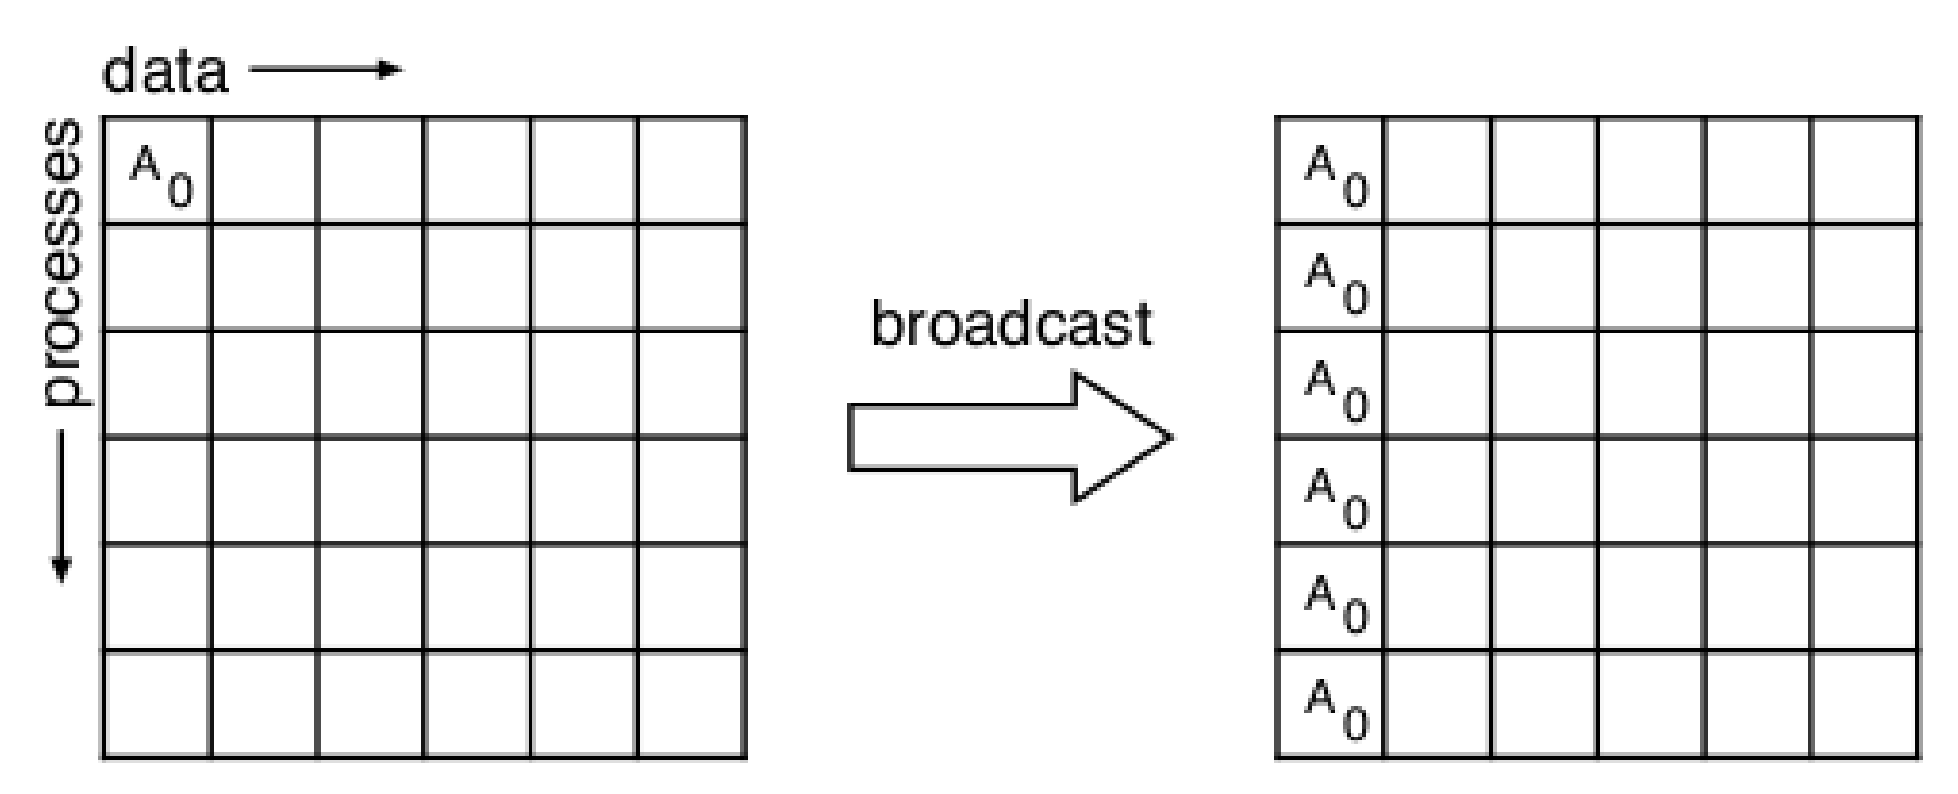
\includegraphics[width=\textwidth]{../figures/broadcast}
     \end{subfigure}
     \\
     \begin{subfigure}[b]{0.8\textwidth}
         \centering
         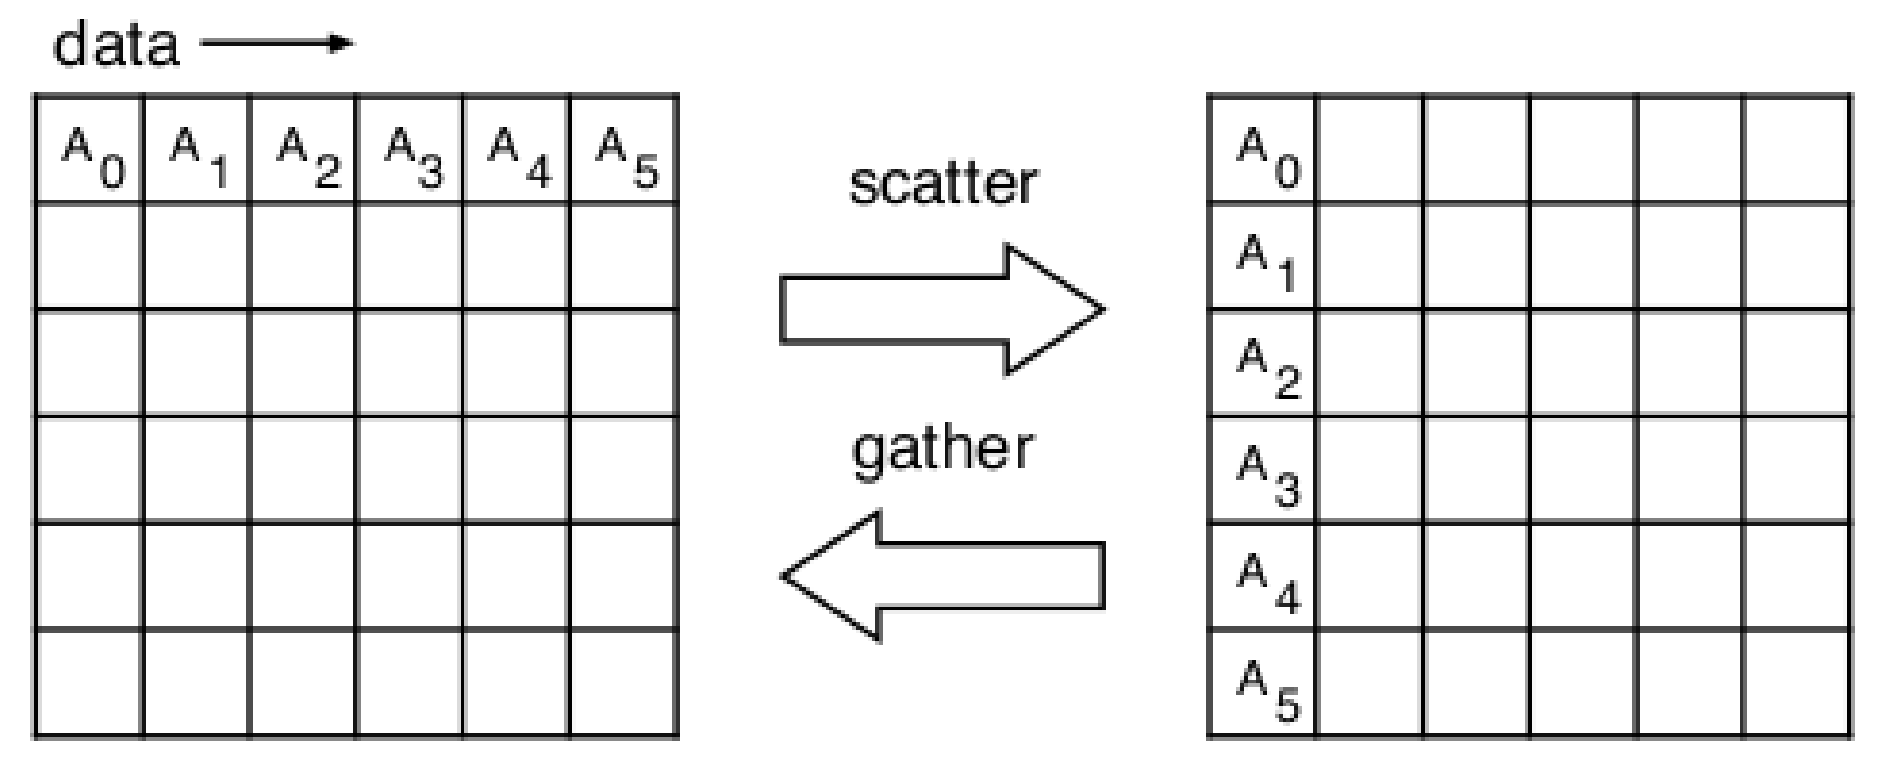
\includegraphics[width=\textwidth]{../figures/scatter}
     \end{subfigure}
\end{figure}
(Sources: \url{https://nyu-cds.github.io/python-mpi/05-collectives/} \\ \url{https://research.computing.yale.edu/sites/default/files/files/mpi4py.pdf})
    \item Consider the multiplication of a matrix $A \in \R^{m \times n}$ with a vector $v \in \R^n$. Write a Python file containing a script that:
    \begin{itemize}
        \item Creates a matrix of dimension $m \times n$
        \item Creates a vector of dimension $n$
        \item Makes sure that the dimensions of the matrix and the vector agree in such way that we can compute $Av$
        \item Computes $Av$ using MPI's scattering, make sure you execute your code on the right amount of processors (\textit{Hints: you'll need to use} |comm.gather|. \textit{What are the entries of $Av$?}) \\
        \lstinputlisting{../build/solution/exercise3_2.py}
    \end{itemize}
\end{enumerate}

{\bf{Exercise IV Collective communication - all-to-all and reduce }}\\

\begin{itemize}
   \item Run the following code on 4 processors:
   \begin{verbatim}
from mpi4py import MPI
import numpy as np

comm = MPI.COMM_WORLD
size = comm.Get_size()
rank = comm.Get_rank()

senddata = rank*np.ones(size, dtype = int)

recvdata = comm.alltoall(senddata)

print(" process ", rank, " sending ", senddata, " receiving ", recvdata )
   \end{verbatim}
   What is |comm.alltoall| doing? Compare it to |comm.scatter|. \\
   |alltoall| combines the scatter and gather functionality. It is better explained in the diagram below.
   \begin{figure}[H]
     \centering
      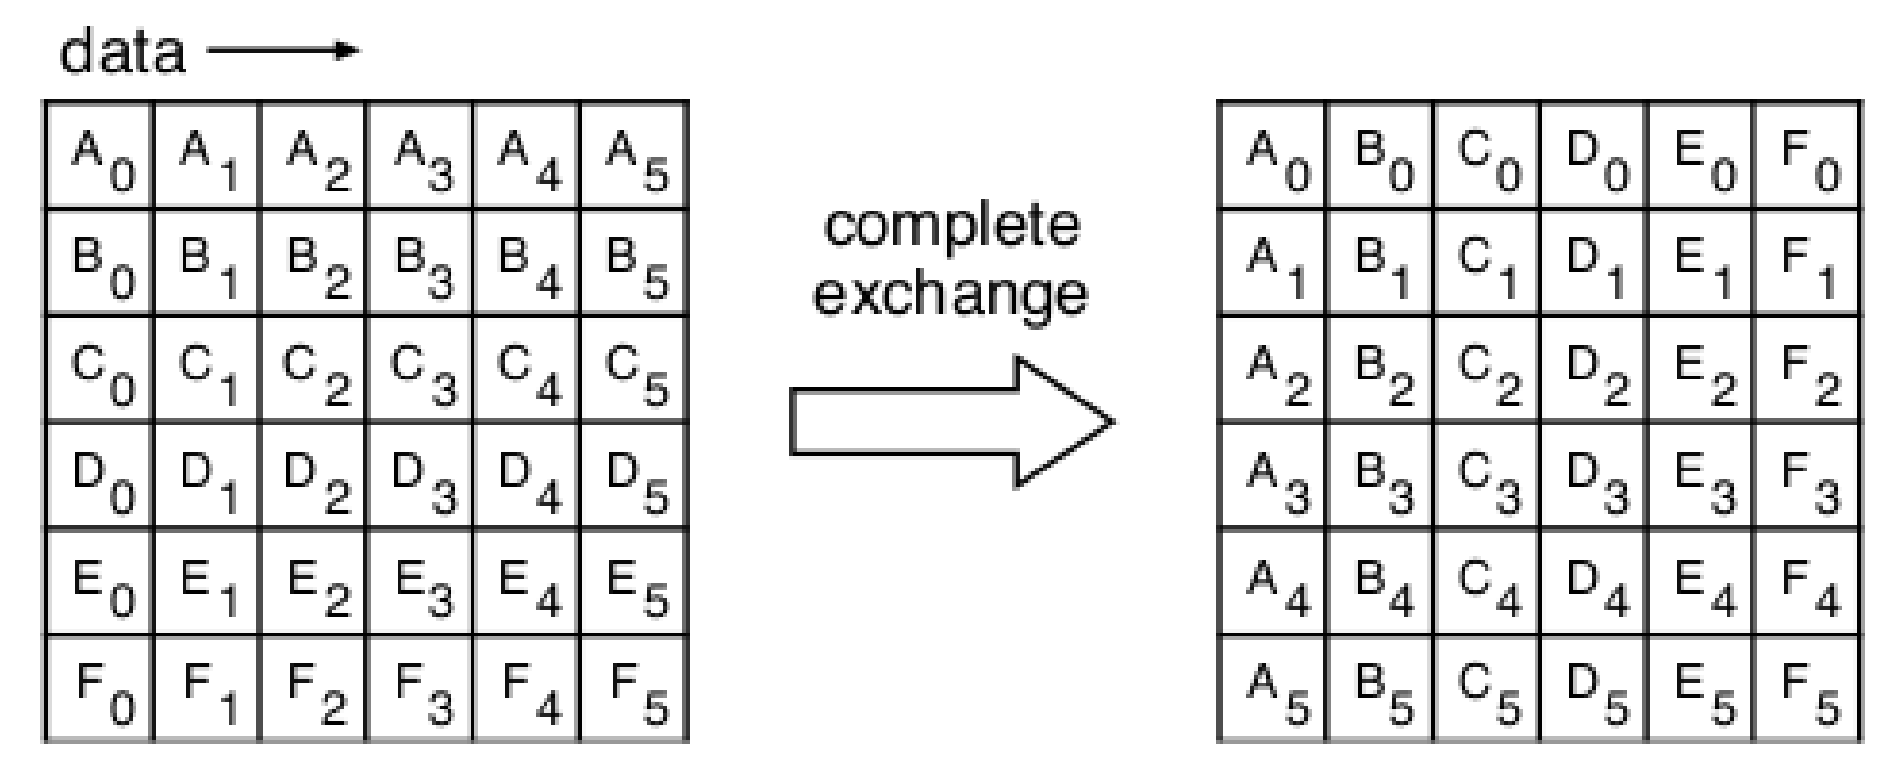
\includegraphics[width=0.8\textwidth]{../figures/alltoall}
\end{figure}
   \item In this exercise we are going to use reduction operations on MPI. Run the following code on 4 processors:
   \begin{verbatim}
from mpi4py import MPI
import numpy as np

comm = MPI.COMM_WORLD
size = comm.Get_size()
rank = comm.Get_rank()

senddata = rank*np.ones(size, dtype = int)

global_result1 = comm.reduce(senddata, op = MPI.SUM, root = 0)
global_result2 = comm.reduce(rank, op = MPI.MAX, root = 0)

#Print
print(" process ", rank, " sending ", senddata)

#Print the result on the root process
if rank == 0:
    print(" Reduction operation1: ", global_result1,
          "\n Reduction operation2: ", global_result2)
   \end{verbatim}
   What is a reduction operation? What is the difference between this and |comm.gather|? \\
   Data reduction involves reducing a set of numbers into a smaller set of numbers via a function. The |comm.reduce| method takes an array of input elements and returns an array of output elements to the root process. The output elements contain the reduced result. MPI contains a set of common reduction operations that can be used, although custom reduction operations can also be defined. 
   (Source: \url{https://nyu-cds.github.io/python-mpi/05-collectives/})
   \item In the previous code, change |comm.reduce| to |comm.allreduce|. What is the difference between the two? (Note, |comm.allreduce| doesn't use the argument |root|). \\
   In |comm.reduce| the output array of the reduction is saved just in the root process but with |comm.allreduce| such output is saved in all the processes. 
   \lstinputlisting{../build/solution/exercise4_3.py}
\end{itemize}


{\bf{Exercise V Deciding what to use - Mid point rule }}\\

Numerical integration describes a family of algorithms for calculating the value of definite integrals. One of the simplest algorithms to do so is called the Mid Point Rule. Assume that $f(x)$ is continous on $[a,b]$. Let $n$ be a positive integer and $h = (b-a)/n$. If $[a,b]$ is divided into $n$ subintervals, $\{ x_0, x_1, ..., x_{n-1} \}$, then if $m_i = (x_{i} + x_{i+1} )/2$ is the midpoint of the i-th subinterval, set:

\[ M_n = \sum_{i=1}^{n} f(m_i)h. \]

Then:

\[ \underset{n \to \infty}{\lim}M_n = \int_a^b f(x) dx. \]

Thus, for a fixed $n$, we can approximate this integral as:

\[ \int_a^b f(x) dx \approx \sum_{i=1}^{n} f(m_i)h  \]

Set $n = s*500$, $f(x) = \cos(x)$, $a = 0$, $b = \pi /2$. Write a Python script such that:
\begin{itemize}
    \item Defines a function that given $x_i, h, n$ first calculates $500$ mid points on a subinterval $[x_{i}, x_{i+1}]$ and returns the approximation of the integral on this subinterval.
    \item Using MPI approximates the integral of $f$ on $[a,b]$
    \item Run your script on $s$ processors
\end{itemize}


to approximate the integral of $f$. (\textit{Hints: there are many ways of doing this, one approach is using } |comm.bcast| \textit{ and } |comm.reduce| ). \\

\lstinputlisting{../build/solution/exercise5.py}

\end{document}
